\section{Initial Experiments}

\subsection{Calibrating and Programming ESCs}
ESCs have 5 input pins, 3 of which come from the flight controller. These 3 wires supply the signal for the ESC to translate into the angle of the shaft for the motor. Before ESCs can be used, they need to be properly calibrated. Programming additional settings is optional, but in most cases necessary too. Normally, the calibration for UAVs is done by setting the throttle to full on the radio controller before powering the ESCs. However, since the board translates the throttle signal into a PWM signal, it is possible to calibrate and run the motors directly from the flight controller by sending a PWM signal using software.

The calibration is done by first sending the maximum length of signal the user wishes to use. The ESC emits sounds that are brand-specific and indicate whether the signal was successfully recognised or not. Once the maximum signal is accepted, the user the emits the minimum signal and waits for approval. Additional sound is then emitted, indicating that the calibration was successful.

Using Arduino's Servo library, a self-explanatory built-in function \textit{servo.writeMicroseconds(int value)} is used to send the signal. By default, the library has the minimum signal set to 544$\mu s$ and the maximum - to 2400$\mu s$. For this project, we shortened the range down to 700$\mu s$ and 2000$\mu s$ for both signals respectively. A commented code used to calibrate the ESC connected to the first pin of the board can be seen in listing \ref{code:calib}.

\lstinputlisting[language=C++, caption={Calibrating the ESC}, label={code:calib}]{Arduino/ESCCalib/ESCCalib.ino}

Programming additional settings of the ESC is done in a similar manner - by sending minimum and maximum signals after the ESC emits particular sounds, indicating wanted selections. The programmable features and selections are brand-specific and can be found in the datasheets. For the purposes of this project, the ESCs have been programmed to include two features - brake mode off and selection of li-ion battery.

\subsection{Expected and Real Motor Performance}
The motors used in the prototype specify to be rated at $K_v$ of 980. $K_v$ is a constant describing the ration between RPM and the applied voltage and is expressed as $K_v = \frac{RPM}{V}$. Derived from this, voltage's effect on the RPM can be seen in figure \ref{KvPlot}.
\begin{figure}[H]
  \centering
    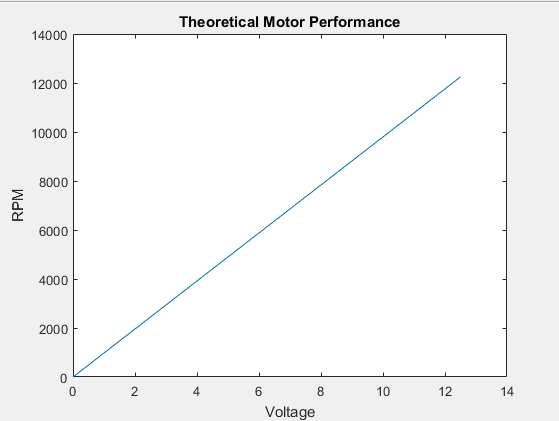
\includegraphics[width=0.8\textwidth]{images/KvPlot.png}
	\caption{Expected motor performance}
	\label{KvPlot}
\end{figure}
With a fully charged battery, the RPM is expected to be $980*11.1V = 10878 RPM$.

In order to confirm this, the actual RPM was measured using SHIMPO DT-205 digital tachometer. A piece of reflective paper was taped to one of the motors so that the tachometer would have something to lock onto, as seen in figure \ref{tachometer}.

\begin{figure}[H]
  \centering
    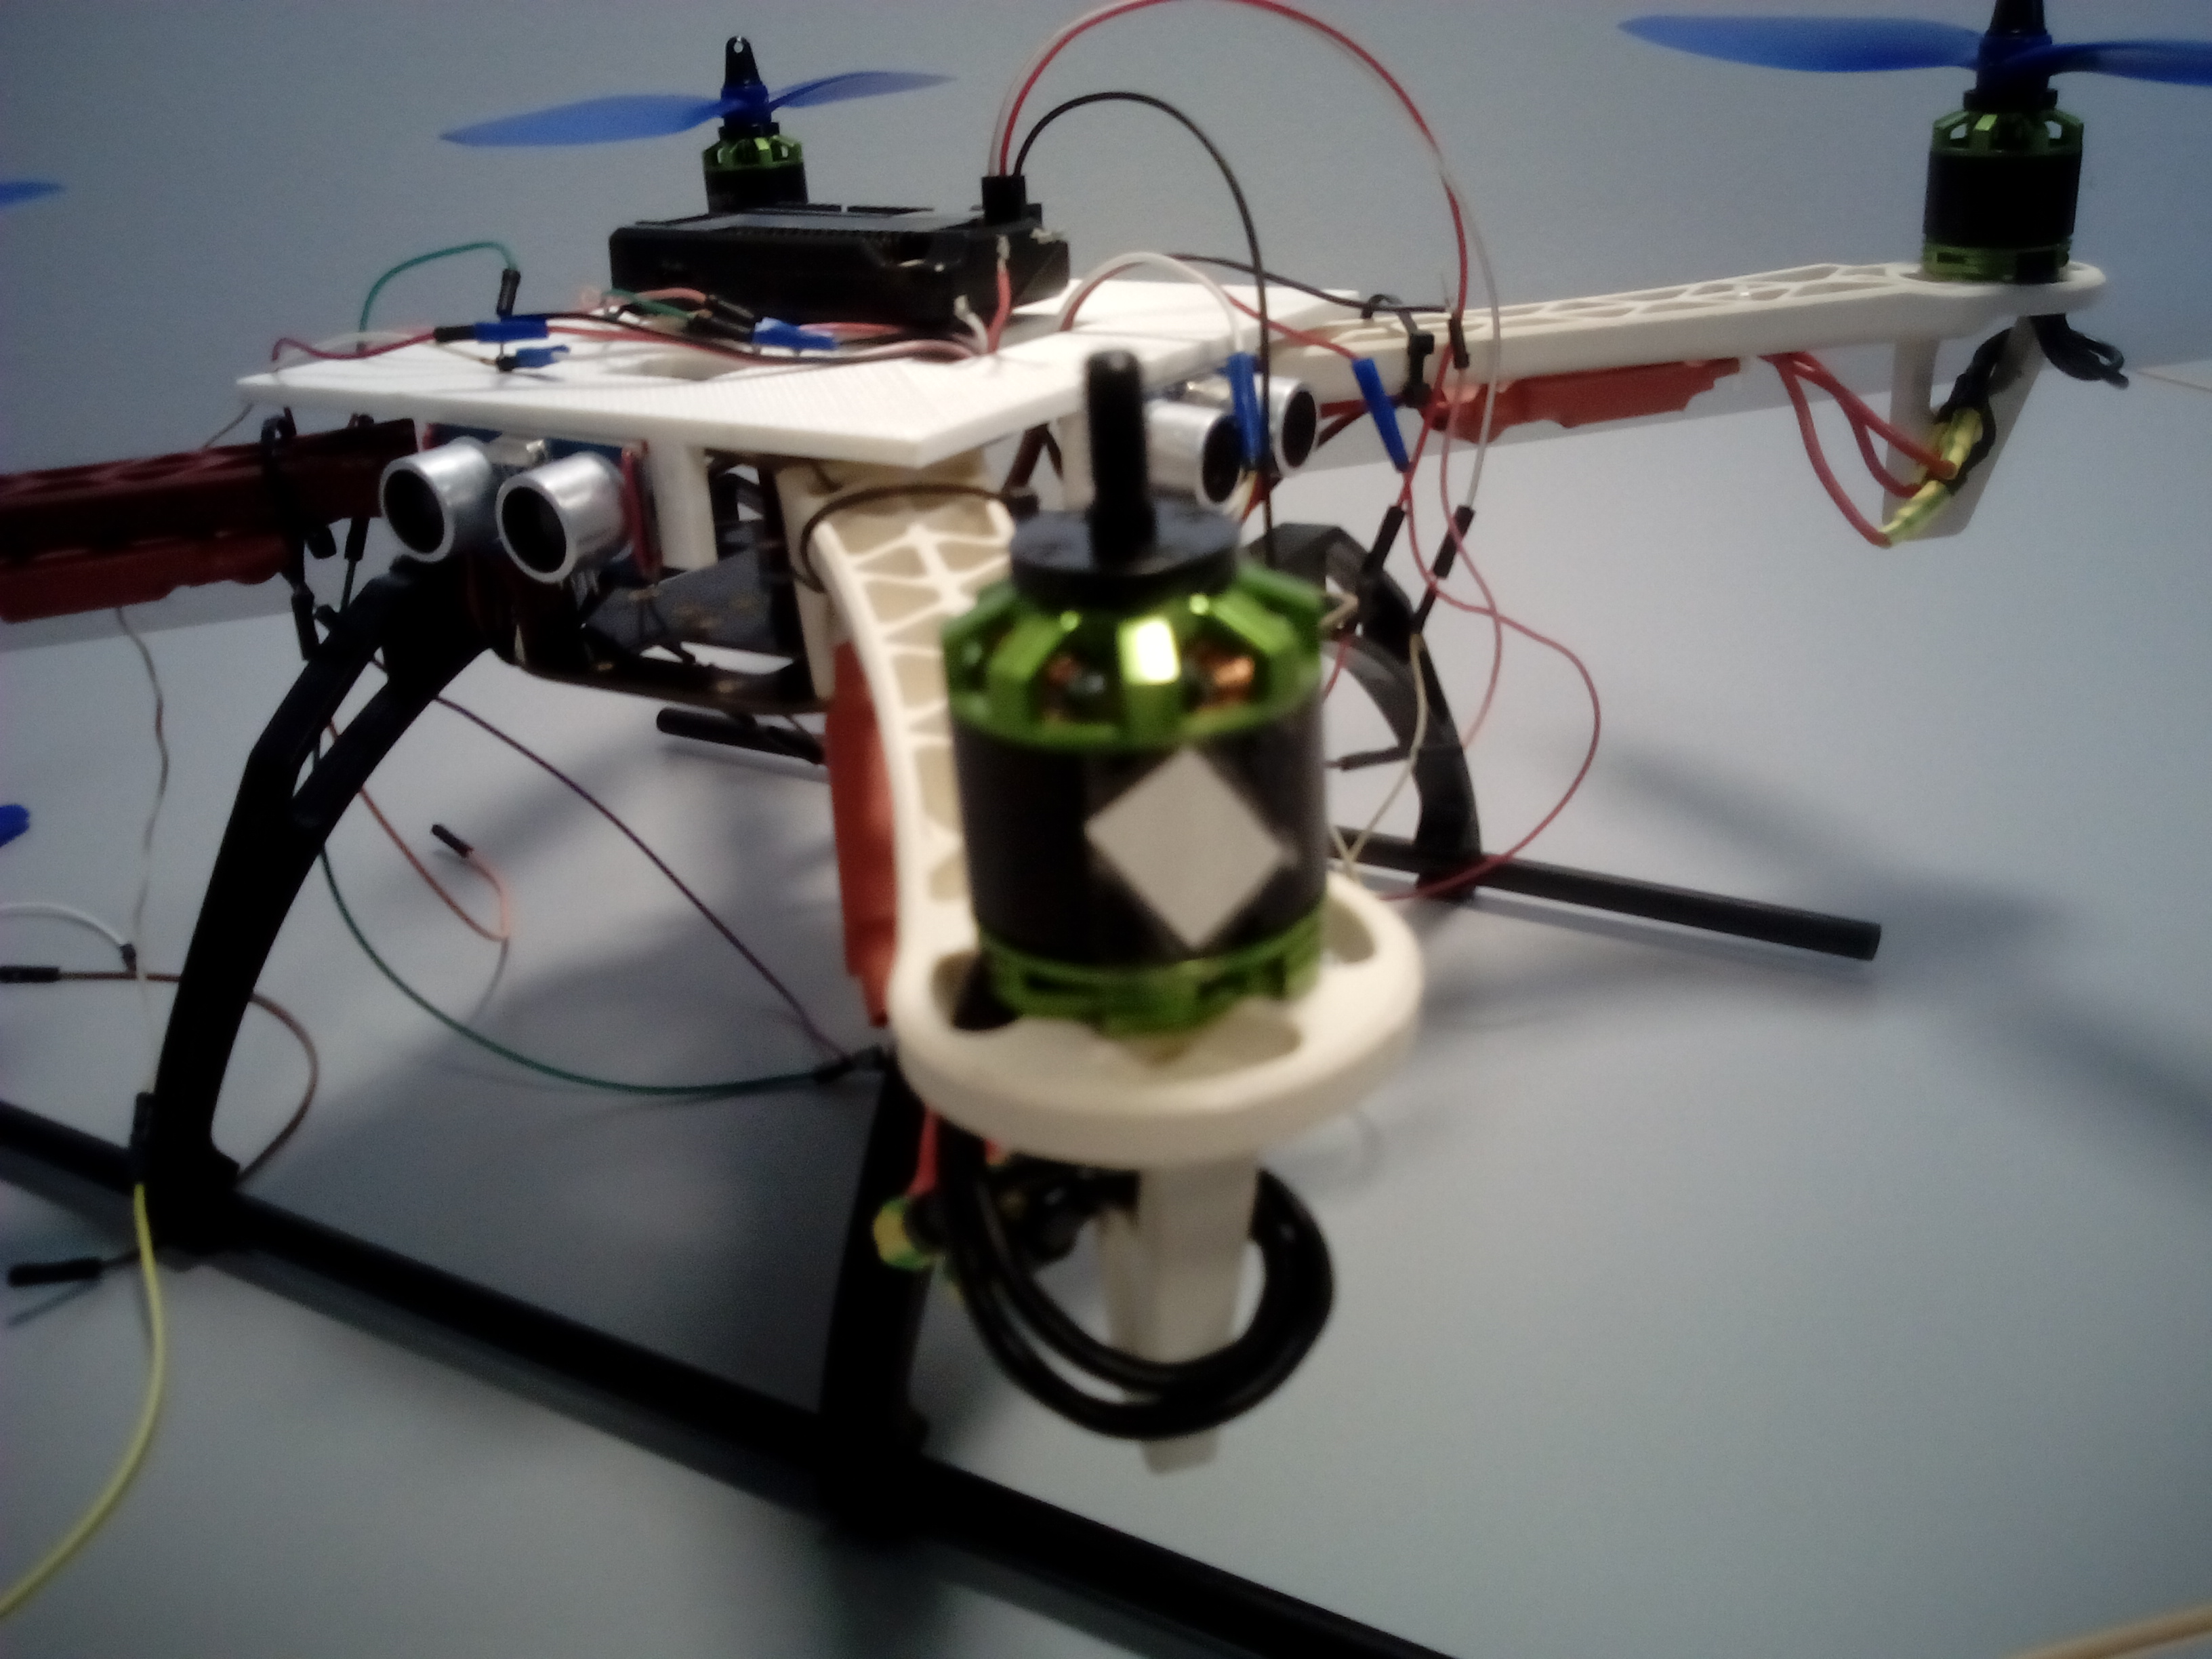
\includegraphics[width=0.5\textwidth]{images/tachometer.jpg}
	\caption{Reflective paper on the motor}
	\label{tachometer}
\end{figure}

By sending the maximum signal from the board, the RPM was measured to be 10812, with a small possible error.
In conclusion, the motors' $K_v$ coefficient found in the datasheet is in fact correct.

\subsection{Output Operating Range}

Since there is no direct translation between the output signal from the board and the speed of the motor and the ESC allows more current than the motor can recognise, it is necessary to find the operating range for the board output that has the most noticeable effect on the RPM of the motor. Through trial and error and by measuring the RPM using SHIMPO DT-205 digital tachometer. The lowest operating point was found to be 762$\mu s$, at which the motor finally begins to spin. The highest point was defined at 1200$\mu s$. Higher values were found to have very small effect on the RPM.
Therefore, despite the ESC recognising the values between 700 and 2000$\mu s$, the most noticeable effect will be between 762 and 1200$\mu s$ and will be primarily used in the project.

\subsection{APM Frequency}
Due to lack of proper documentation, it was necessary to do measure the frequency of the signals sent out by the flight controller. To do so, an oscilloscope was connected to one of the output pins of the board. Then, using the servo library, a signal was sent out. The interval between signals was found to be 20$ms$, therefore, the frequency of the board is 50$Hz$, as seen in figure \ref{oscillo1}.
\begin{figure}[H]
  \centering
    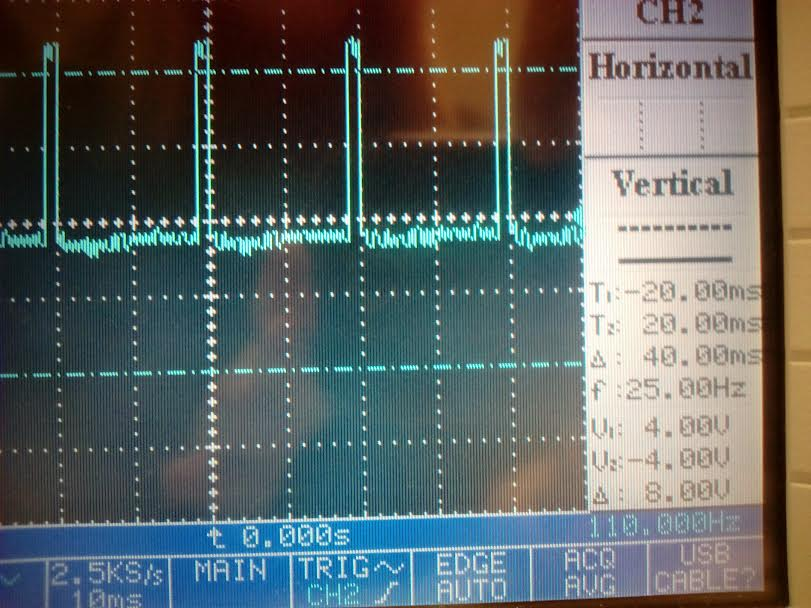
\includegraphics[width=0.5\textwidth]{images/oscillo1.jpg}
	\caption{Oscilloscope measuring APM's frequency}
	\label{oscillo1}
\end{figure}

The second experiment on the board was then made to determine how the flight controller handles the output signals during those 20$ms$. First two outputs of the APM were connected to the oscilloscope, both utilizing the Servo library to send signals of length of 2000$\mu s$. Results can be seen in figure \ref{oscillo2}.
\begin{figure}[H]
  \centering
    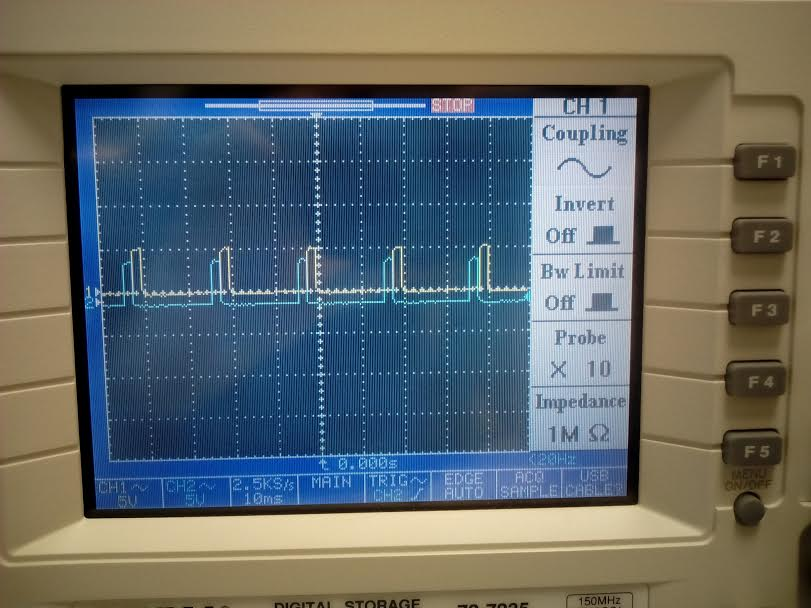
\includegraphics[width=0.5\textwidth]{images/oscillo2.jpg}
	\caption{Readings of the two output signals}
	\label{oscillo2}
\end{figure}

Then, for further testing purposes, both outputs were given different values in two scenarios, as seen in figure \ref{oscillo3}.

\begin{figure}[H]
  \centering
    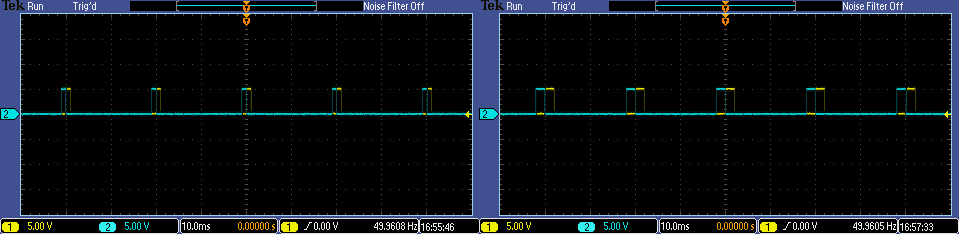
\includegraphics[width=0.5\textwidth]{images/oscillo3.png}
	\caption{Left - signals running at 2000$\mu s$; Right - 700$\mu s$}
	\label{oscillo3}
\end{figure}

From this, two conclusions can be made:
\begin{enumerate}
\item If the first signal is shorter than the second one, the second signal will still follow right after the first signal ends. In other words, the APM leaves no gaps between the outputs.
\item Since the board runs at the frequency of 50$Hz$ and has a period of 20$ms$, this leaves $\frac{20}{8} = 2.5ms$ maximum length for each output signal. The servo library is hard-capped at 2.4$ms$ and thus is well within the limits of the board.
\end{enumerate}

\subsection{Estimating Motor Coefficients}
Kt
KT
Ke

\subsection{APM Output and ESC Output Relationship}

In order to use the board's output signal as an input in a mathematical model, it is necessary to find an equation to translate it into an angular rate.
First, an equation has been found that describes the relationship between motor's RPM, ESC's output signal frequency and number of motor poles \cite{RPMEq}:
\begin{equation}
\label{voltage1}
	RPM = \frac{120*f}{n}
\end{equation}
Here, $f$ is the frequency and $n$ is the number of poles (in this case - 14).

Therefore, it is possible to measure the frequency at various output values, which can then be used to define an equation that uses the board's signal length as an input value and results in an RPM.

INPUT AND FREQUENCY TABLE, TRANSLATED INTO RPM FOR EASIER COMPARISON

To verify these values, RPM was manually measured using the tachometer at same output values, as seen in table \ref{RPMTable}.

\begin{table}[H]
\centering
\begin{tabular}{|c|c|}
\hline
$Output value$ 	& $RPM$ \\ \hline
762 			& 2700	\\ \hline
800 			& 4640  \\ \hline
810 			& 5167	\\ \hline
820 			& 5638  \\ \hline
830				& 6000 	\\ \hline
840				& 6314	\\ \hline
850 			& 6580	\\ \hline
860 			& 6890	\\ \hline
870 			& 7134	\\ \hline
880 			& 7368	\\ \hline
890 			& 7582	\\ \hline
900 			& 7777	\\ \hline
925 			& 8305	\\ \hline
950 			& 8635	\\ \hline
975 			& 8955	\\ \hline
1000 			& 9190	\\ \hline
1050 			& 9611	\\ \hline
1100 			& 9896	\\ \hline
1150 			& 10120	\\ \hline
1200			& 10100	\\ \hline
\end{tabular}
\caption{RPM measured at different values}
\label{RPMTable}
\end{table}

The two tables \ref{RPMTable} and \ref{FreqTable} were then plotted to see the difference, which are seen in figure \ref{RPMvsFreq}.
PLACEHOLDER FIGURE
\begin{figure}[H]
  \centering
    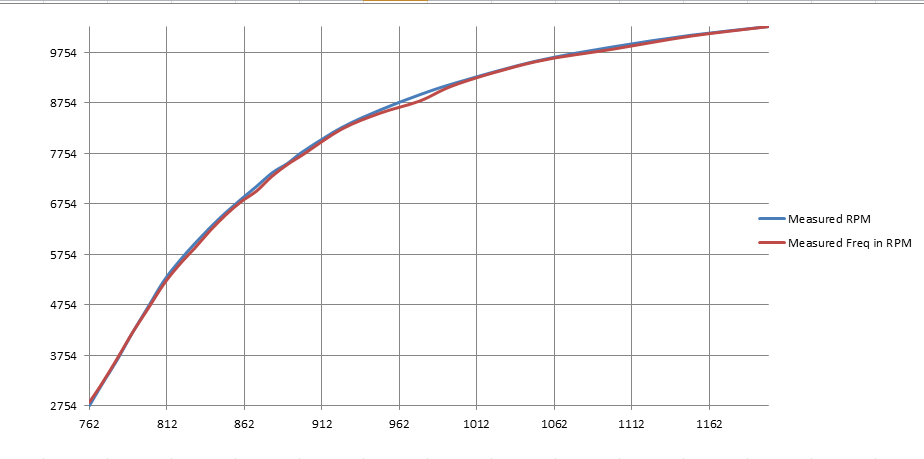
\includegraphics[width=0.8\textwidth]{images/RPMvsFreq.png}
	\caption{Plotted values of manually measured and frequency-based RPM}
	\label{RPMvsFreq}
\end{figure}

TALK ABOUT COMPARISON, DERIVE AN EQUATION